%MCQMC, April 6-11, 2014
%Requires graphics files
%  Lattice64.eps, DualLattice64.eps, PlotFFTCoefUse256.eps, geomeancubLatticeErrTime_d_64.eps

%%%%%%%%%%%%%%%% Springer %%%%%%%%%%%%%%%%%%%%%%%%%%%%%%%%%%
\documentclass[graybox]{svmult}

\smartqed
\usepackage{mathptmx}       % selects Times Roman as basic font
\usepackage{helvet}         % selects Helvetica as sans-serif font
\usepackage{courier}        % selects Courier as typewriter font
\usepackage{type1cm}        % activate if the above 3 fonts are
                            % not available on your system
\usepackage{graphicx}       % standard LaTeX graphics tool
                            % when including figure files

\usepackage{array,colortbl}
\usepackage{amsmath,amsfonts,amssymb,bm} % no amsthm, Springer defines Theorem, Lemma, etc themselves
%\usepackage[mathx]{mathabx}
\DeclareFontFamily{U}{mathx}{\hyphenchar\font45}
\DeclareFontShape{U}{mathx}{m}{n}{
      <5> <6> <7> <8> <9> <10>
      <10.95> <12> <14.4> <17.28> <20.74> <24.88>
      mathx10
      }{}
\DeclareSymbolFont{mathx}{U}{mathx}{m}{n}
\DeclareFontSubstitution{U}{mathx}{m}{n}
\DeclareMathAccent{\widecheck}      {0}{mathx}{"71}

% Note that Springer defines the following already:
%
% \D upright d for differential d
% \I upright i for imaginary unit
% \E upright e for exponential function
% \tens depicts tensors as sans serif upright
% \vec depicts vectors as boldface characters instead of the arrow accent
%
% Additionally we throw in the following common used macro's:
\newcommand{\Z}{\mathbb{Z}} % integers
\newcommand{\C}{\mathbb{C}} % complex numbers
\newcommand{\R}{\mathbb{R}} % reals
\newcommand{\N}{\mathbb{N}} % natural numbers {1, 2, ...}
\newcommand{\Q}{\mathbb{Q}} % rationals
\newcommand{\F}{\mathbb{F}} % field, finite field
\newcommand{\floor}[1]{\left\lfloor #1 \right\rfloor} % floor
\newcommand{\ceil}[1]{\left\lceil #1 \right\rceil}    % ceil
\newcommand{\rd}{\,\mathrm{d}} % differential symbol for use in integrals
% vectors as boldsymbols:
\newcommand{\bszero}{\boldsymbol{0}} % vector of zeros
\newcommand{\bsone}{\boldsymbol{1}}  % vector of ones
\newcommand{\bst}{\boldsymbol{t}}    % vector t
\newcommand{\bsu}{\boldsymbol{u}}    % vector u
\newcommand{\bsv}{\boldsymbol{v}}    % vector v
\newcommand{\bsw}{\boldsymbol{w}}    % vector w
\newcommand{\bsx}{\boldsymbol{x}}    % vector x
\newcommand{\bsy}{\boldsymbol{y}}    % vector y
\newcommand{\bsz}{\boldsymbol{z}}    % vector z
\newcommand{\bsDelta}{\boldsymbol{\Delta}}    % vector \Delta
% sets as Euler fraks:
\newcommand{\setu}{\mathfrak{u}}
\newcommand{\setv}{\mathfrak{v}}
% indicator boldface 1:
\DeclareSymbolFont{bbold}{U}{bbold}{m}{n}
\DeclareSymbolFontAlphabet{\mathbbold}{bbold}
\newcommand{\ind}{\mathbbold{1}}


\usepackage{microtype} % good font tricks

\usepackage[colorlinks=true,linkcolor=black,citecolor=black,urlcolor=black]{hyperref}
\urlstyle{same}
\usepackage{bookmark}
\pdfstringdefDisableCommands{\def\and{, }}
\makeatletter % to avoid hyperref warnings:
  \providecommand*{\toclevel@author}{999}
  \providecommand*{\toclevel@title}{0}
\makeatother

%Fred's additions
%
\usepackage{mathtools,array,booktabs,xspace}
\DeclareMathOperator{\ok}{ok}

%%%%%%%%%%%%%%%%%%%%%%%%%%%%%%%%%%%%%%%%%%%%%%%%%%%%%%%%%%%%%%%%%%%%%%%%%%%%%%%%%%%%%%%%%
\begin{document}
\spnewtheorem{algo}{Algorithm}{\bf}{\rm}
\newcommand{\bsa}{\boldsymbol{a}}    %%% vector a
\newcommand{\bsh}{\boldsymbol{h}}    %%% vector h
\newcommand{\bsi}{\boldsymbol{i}}    % vector i
\newcommand{\bsj}{\boldsymbol{j}}    %%% vector j
\newcommand{\bsk}{\boldsymbol{k}}    % vector k
\newcommand{\bsl}{\boldsymbol{l}}    % vector l
\newcommand{\bsr}{\boldsymbol{r}}    % vector r
\newcommand{\bsnu}{\boldsymbol{\nu}}    % vector nu
\newcommand{\dif}{{\rm d}}			%%% Differential dx
\newcommand{\me}{\text{e}}			%%% Do not
\newcommand{\cc}{\mathcal{C}}
\newcommand{\cm}{\mathcal{M}}		%%%
\newcommand{\cl}{\mathcal{L}}
\newcommand{\cn}{\mathcal{N}}
\newcommand{\Order}{\mathcal{O}}
\newcommand{\cp}{\mathcal{P}}
\newcommand{\cx}{\mathcal{X}}
\newcommand{\natm}{\N_{0,m}}
\newcommand{\cube}{[0,1)^d}
\newcommand{\hf}{\hat{f}}
\newcommand{\rf}{\mathring{f}}
\newcommand{\tf}{\tilde{f}}
\newcommand{\hg}{\hat{g}}
\newcommand{\hI}{\hat{I}}
\newcommand{\tvk}{\tilde{\bsk}}
\newcommand{\hS}{\widehat{S}}
\newcommand{\tS}{\widetilde{S}}
\newcommand{\wcS}{\widecheck{S}}
\newcommand{\okappa}{\overline{\kappa}}
\newcommand{\rnu}{\mathring{\nu}}
\newcommand{\tnu}{\widetilde{\nu}}
\newcommand{\hnu}{\widehat{\nu}}
\newcommand{\onu}{\overline{\nu}}
\newcommand{\hbsnu}{\widehat{\bsnu}}   %%%
\newcommand{\homega}{\widehat{\omega}}
\newcommand{\wcomega}{\mathring{\omega}}
\newcommand{\fC}{\mathfrak{C}}
\newcommand{\nodes}{\{\bsz_i\}_{i=0}^{\infty}}
\newcommand{\nodesn}{\{\bsz_i\}_{i=0}^{n-1}}
\newcommand{\norm}[1]{\ensuremath{\left \lVert #1 \right \rVert}}
\newcommand{\abs}[1]{\ensuremath{\left |  #1 \right |}} %%%
\newcommand{\bigabs}[1]{\ensuremath{\bigl \lvert #1 \bigr \rvert}}
\newcommand{\Bigabs}[1]{\ensuremath{\Bigl \lvert #1 \Bigr \rvert}}
\newcommand{\biggabs}[1]{\ensuremath{\biggl \lvert #1 \biggr \rvert}}
\newcommand{\Biggabs}[1]{\ensuremath{\Biggl \lvert #1 \Biggr \rvert}}
\newcommand{\ip}[3][{}]{\ensuremath{\left \langle #2, #3 \right \rangle_{#1}}}

\newcommand{\lattice}{\cl} %you can make your own here
\newcommand{\Lebesgue}{L} %you can make your own here

\allowdisplaybreaks

\title*{Adaptive Multidimensional Integration Based on Rank-1 Lattices}
\author{Llu\'is Antoni Jim\'enez Rugama \and Fred J. Hickernell}
\institute{Llu\'is Antoni \and Fred J. Hickernell \at Department of Applied Mathematics,  Illinois Institute of Technology, 10 W. 32$^{\text{nd}}$ Street, E1-208, Chicago, IL 60616, USA
\email{ljimene1@hawk.iit.edu},\email{hickernell@iit.edu}}
\maketitle

\abstract{Quasi-Monte Carlo methods are used for numerically integrating multivariate functions. However, the error bounds for these methods typically rely on a priori knowledge of some semi-norm of the integrand, not on the sampled function values. In this article, we propose an error bound based on the discrete Fourier coefficients of the integrand. If these Fourier coefficients decay more quickly, the integrand has less fine scale structure, and the accuracy is higher. We focus on rank-1 lattices because they are a commonly used quasi-Monte Carlo design and because their algebraic structure facilitates an error analysis based on a Fourier decomposition of the integrand. This leads to a guaranteed adaptive cubature algorithm with computational cost $\Order(mb^m)$, where $b$ is some prime number and $b^m$ is the number of data points.}

\section{Introduction}

Quasi-Monte Carlo (QMC) methods use equally weighted sums of integrand values at carefully chosen nodes,
\[
\frac 1n \sum_{i=0}^{n-1} f(\bsz_i), 
\]
to approximate multidimensional integrals over the unit cube,
\[
\int_{\cube} f(\bsx) \, \dif \bsx.
\]
Integrals over more general domains may often be accommodated by a transformation of the integration variable. QMC methods are widely used because they do not suffer from a \textit{curse of dimensionality}. For example, if $d \ge 5$, QMC methods with an error of $\Order(n^{-(1-\delta)})$ have a faster convergence rate than the tensor product composite Simpson's rule, which has error of $\Order(n^{-4/d})$. Assumptions under which the strong tractability of QMC methods occur can be found in \cite{HicWoz99}.

The convergence rate $\Order(n^{-(1-\delta)})$ does not give enough information about the absolute error to determine how large $n$ must be to satisfy a given error tolerance, $\varepsilon$. The objective of this research is to develop a guaranteed, QMC algorithm based on rank-1 lattices that determines $n$ adaptively by calculating a data-driven upper bound on the absolute error. The Koksma-Hlawka inequality is impractical for this purpose because it requires the total variation of the integrand. Our data-driven bound is expressed in terms of the integrand's discrete Fourier coefficients. 

Sections \ref{secrank1lat} and \ref{secfourierseries}, describe the group structure of rank-1 lattices and how the complex exponential functions are an appropriate basis for these nodes. For computation purposes, there is also an explanation of how to obtain the discrete Fourier transform of $f$ via a Fast Fourier Transform, with an $\Order(n \log(n))$ computational cost.  The new contributions are described in Section \ref{secalgo}. Initially, a mapping from $\N$ to the space of wavenumbers, $\Z^d$, is defined according to constraints given by the structure of our nodes. With this mapping, we define a set of integrands for which our new adaptive algorithm is designed.  This set is defined in terms of cone conditions satisfied by the Fourier coefficients of the integrands. These conditions make it possible to derive an upper bound on the rank-1 lattice rule error in terms of the discrete Fourier coefficients, which can be used to construct an adaptive algorithm.  An upper bound on the computational cost of this algorithm is derived. Finally, there is an example of option pricing using the MATLAB implementation of our algorithm, \texttt{cublattice\_g}, which will appear in the next release of the Guaranteed Automatic Integration Library \cite{ChoEtal14a}.  A parallel development for Sobol' cubature is given in \cite{HicJim16a}.

\section{Rank-1 Integration Lattices}\label{secrank1lat}

Let $b$ be prime number, and let $\F_{n}:=\{0, \ldots, n-1\}$ denote the set of the first $n$ non-negative integers for any $n \in \N$. The aim is to construct a sequence of embedded node sets with $b^m$ points for $m \in \N_0$:
\[
\{\bszero\}=:\cp_0\subset \cp_1 \dots\subset\cp_m:=\{\bsz_i\}_{i=0}^{b^m-1} \subset\dots\subset\cp_\infty:=\{\bsz_i\}_{i=0}^{\infty}.
\]
Specifically, the sequence $\bsz_1, \bsz_b, \bsz_{b^2},  \ldots \in \cube$ is chosen such that 
\begin{subequations} \label{zbmdef}
\begin{gather} 
\bsz_1 = b^{-1} \bsa_1, \qquad \bsa_1 \in \{1, \ldots, b-1\}^{d}, \\
\bsz_{b^m} = b^{-1}(\bsz_{b^{m-1}}+\bsa_m)= b^{-1}\bsa_m + \cdots + b^{-m} \bsa_1, \qquad \bsa_m \in \F_b^{d}, \quad m \in \N\setminus\{1\}.
\end{gather}
\end{subequations}
From this definition it follows that
\begin{equation} 
b\bsz_{b^m} \bmod {1} =\bsz_{b^{m-1}}, \quad b^{m}\bsz_{b^{m}} \bmod {1} = \bszero \qquad \forall m \in \N ,\label{latpropb}
\end{equation}
Next, for any $i \in \N$ with proper $b$-ary expansion $i=i_0+i_1 b + i_2 b^2 + \cdots$, and $m=\lfloor \log_b(i) \rfloor+1$ define 
\begin{multline} \label{zidef}
\bsz_i : = \sum_{\ell=0}^{\infty} i_\ell \bsz_{b^\ell} \bmod 1 = \sum_{\ell=0}^{m-1} i_\ell \bsz_{b^\ell} \bmod 1 = \sum_{\ell=0}^{m-1} i_\ell b^{m-1-\ell}  \bsz_{b^{m-1}} \bmod 1 \\ 
 = j \bsz_{b^{m-1}} \bmod 1, \qquad \text{where } j= \sum_{\ell=0}^{m-1} i_\ell b^{m-1-\ell},
\end{multline}
where \eqref{latpropb} was used.  This means that node set $\cp_m$ defined above may be written as the integer multiples of the generating vector $\bsz_{b^{m-1}}$ since 
\[
\cp_m:= \{\bsz_i\}_{i=0}^{b^m-1} = \bigg \{ \bsz_{b^{m-1}} \sum_{\ell=0}^{m-1} i_\ell b^{m-1-\ell} : i_0, \ldots , i_{m-1} \in \F_b \bigg \} = \left\{ j \bsz_{b^{m-1}} : j \in \F_{b^m} \right \}.
\]

Integration lattices, $\lattice$, are defined as discrete groups in $\R^d$ containing $\Z^d$ and closed under normal addition \cite[Sec. 2.7-2.8]{SloJoe94}.  The node set of an integration lattice is its intersection with the half-open unit cube, $\cp:=\lattice \cap \cube$. In this case, $\cp$ is also a group, but this time under addition modulo 1, i.e., the addition operator $\oplus:\cube \times \cube \to \cube$ defined by $\bsx\oplus\bsy:=\bsx+\bsy\bmod 1$, and where $\ominus \bsx:=\bsone-\bsx$.

The sets $\cp_m$ defined above are embedded node sets of integration lattices. The sufficiency of a single generating vector for each $\cp_m$ is the reason that $\cp_m$ is called the node set of a rank-1 lattice. 
The theoretical properties of good embedded rank-1 lattices for cubature are discussed in \cite{HicNie03a}.  
 
The set of $d$-dimensional integer vectors, $\Z^d$, is used to index Fourier series expressions for the integrands, and $\Z^d$ is also known as the wavenumber space. We define the bilinear operation $\ip{\cdot}{\cdot}: \Z^d \times \cube \to [0,1)$ as the dot product modulo $1$: 
\begin{equation}\label{bilinear}
\ip{\bsk}{\bsx}:=\bsk^T\bsx\bmod 1 \qquad \forall \bsk \in \Z^d, \ \bsx \in \cube.
\end{equation}
This bilinear operation has the following properties: for all $\bst, \bsx \in \cube$, $\bsk, \bsl \in \Z^d$, and $a \in \Z$, it follows that
\begin{subequations}
\begin{gather}
\ip{\bsk}{\bszero} = \ip{\bszero}{\bsx} = 0,\\
\ip{\bsk}{a \bsx \bmod 1 \oplus \bst} = a\ip{\bsk}{\bsx} + \ip{\bsk}{\bst} \bmod 1 \label{bilinearlinxprop} \\
\ip{a \bsk + \bsl}{\bsx} = a\ip{\bsk}{\bsx} + \ip{\bsl}{\bsx} \bmod 1, \label{bilinearlinkprop}\\
\ip{\bsk}{\bsx} = 0 \ \forall \bsk \in \Z^d \ \implies \ \bsx=\bszero.\label{bilinearlinzeroprop}
\end{gather}
\end{subequations}
An additional constraint placed on the embedded lattices is that
\begin{equation}
\ip{\bsk}{\bsz_{b^m}} =  0 \ \forall m \in \N_0   \ \implies \ \bsk=\bszero. \label{latpropd}
\end{equation}

The bilinear operation dedined in \eqref{bilinear} is also used to define the \emph{dual} lattice corresponding to $\cp_m$:
\begin{align}
\nonumber
\cp^{\perp}_m & := \{\bsk \in \Z^d : \ip{\bsk}{\bsz_i} = 0, \ i=0, \ldots, b^m-1\} \\
&= \{\bsk \in \Z^d : \ip{\bsk}{\bsz_{b^{m-1}}} = 0 \} \qquad \text{by \eqref{zidef} and \eqref{bilinearlinxprop}} .\label{dualdef}
\end{align}
By this definition $\cp^{\perp}_{0}=\Z^d$, and the properties \eqref{latpropb}, \eqref{bilinear}, and \eqref{latpropd}, imply also that the $\cp^{\perp}_m$ are nested subgroups with
\begin{equation}\label{dualemb}
\Z^d=\cp^{\perp}_{0}\supseteq\dots\supseteq\cp^{\perp}_{m}\supseteq\dots\supseteq\cp^{\perp}_{\infty}=\{\bszero\}.
\end{equation}

For finite node $m$ the dual lattice $\cp^{\perp}_{m}$ contains infinitely many points. Figure \ref{Latticefig} shows an example of a rank-1 lattice node set with $64$ points in dimension $3$ and its dual lattice. The parameters defining this node set are is $b=2$, $m=6$, and $\bsz_{32}=(1,27,15)/64$.
\begin{figure}[h!]
\centering
\begin{tabular}{>{\centering}p{5cm}>{\centering}p{5cm}}
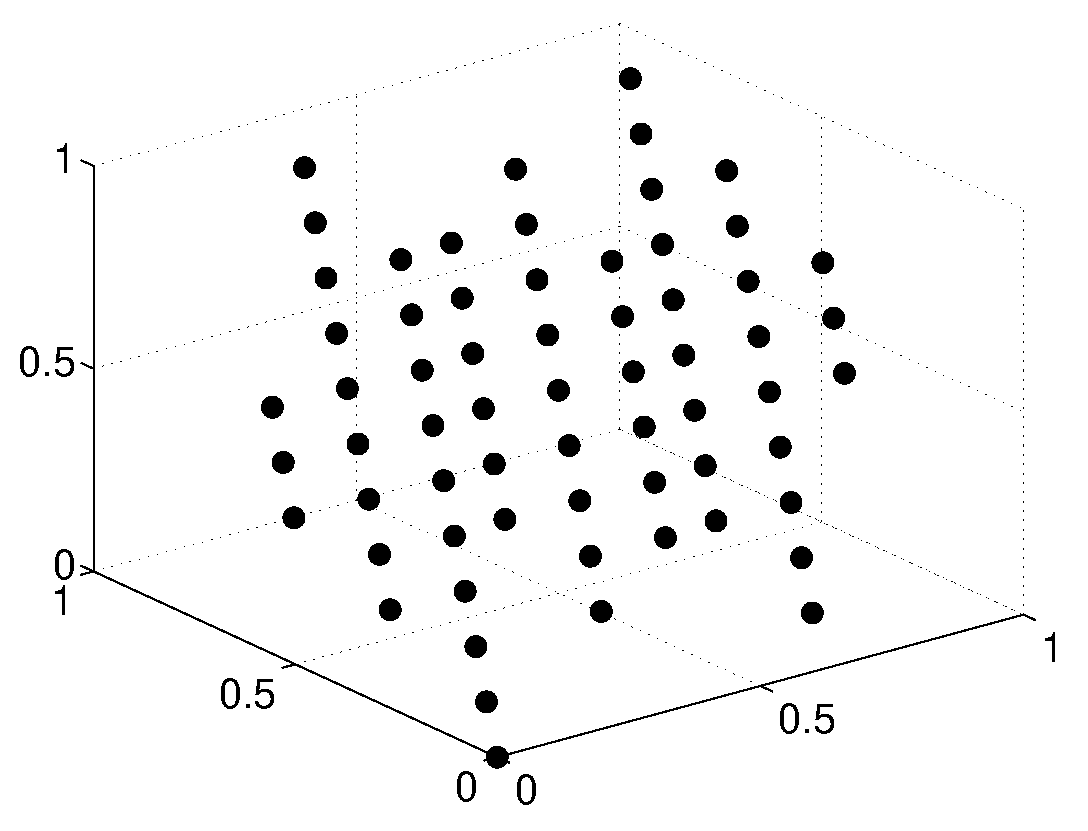
\includegraphics[width=5cm]{Images/Lattice64.eps} &
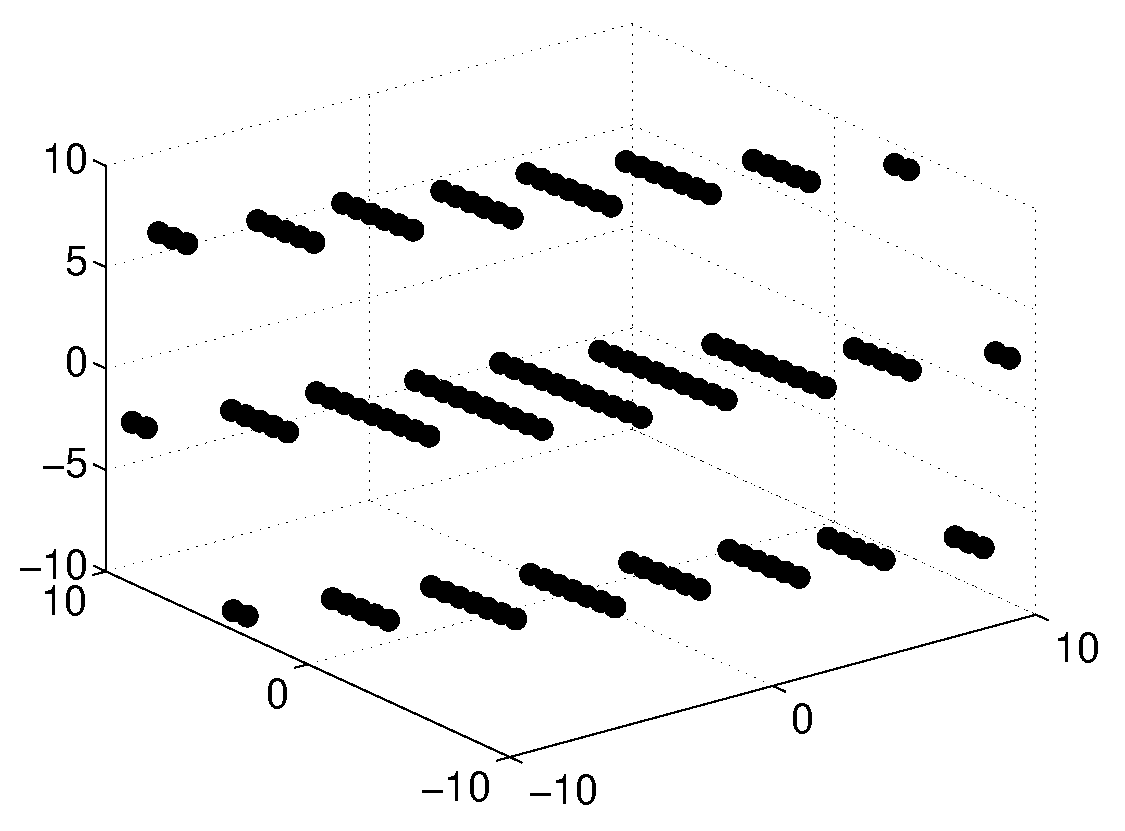
\includegraphics[width=5cm]{Images/DualLattice64.eps}\tabularnewline
a) & b)
\end{tabular}
\caption{Plots of a) the node set $\cp_6$, and b) some of the dual lattice, $\cp_6^{\perp} \cap [-10,10]^3$.}\label{Latticefig}
\end{figure}

\section{Fourier Series}\label{secfourierseries}

The integrands considered here are absolutely continuous periodic functions. If the integrand is not initially periodic, it may be periodized as discussed in \cite{Hic01a}, \cite[Sec. 2.12]{SloJoe94} or \cite{Sid93}. More general box domains may be considered, also by using variable transformations, see e.g.,  \cite{HicSloWas03a,HicSloWas03e}.

The $\Lebesgue_2$ inner product is defined as
\[
\ip[2]{f}{g} = \int_{\cube} f(\bsx) \overline{g(\bsx)} \, \dif \bsx.
\]
The complex exponential functions, $\{\E^{2 \pi \sqrt{-1} \ip{\bsk}{\cdot}}\}_{\bsk \in \Z^d}$ form a complete orthonormal \emph{basis} for $\Lebesgue_2(\cube)$. Then, any function in $\Lebesgue_2$ may be written in series form as
\begin{equation} \label{Fourierdef}
f(\bsx) = \sum_{\bsk \in \Z^d} \hf(\bsk) \E^{2 \pi \sqrt{-1} \ip{\bsk}{\bsx}}, \quad \text{where } \hf(\bsk) = \ip[2]{f}{\E^{2 \pi \sqrt{-1} \ip{\bsk}{\cdot}}},
\end{equation}
and the inner product of two functions in $\Lebesgue_2$ is the $\ell_2$ inner product of their series coefficients:
\[
\ip[2]{f}{g} = \sum_{\bsk \in \Z^d} \hf(\bsk)\overline{\hg(\bsk)} =: \ip[2]{\bigl(\hf(\bsk)\bigr)_{\bsk \in \Z^d}}{\bigl ( \hg(\bsk)\bigr )_{\bsk \in \Z^d}}.
\]

Note that for any $\bsz\in\cp_m$ and $\bsk\in\cp_m^\perp$, we have that $\E^{2 \pi \sqrt{-1} \ip{\bsk}{\bsz}}=1$. The special group structure of the  lattice node set, $\cp_m$, leads to a useful formula for the average of any Fourier basis function over $\cp_m$. For all $\bsk \in \Z^d$ and $\bsz \in \cp_m$, it follows that
\begin{align*}
\nonumber
0 &
= \frac{1}{b^m} \sum_{i=0}^{b^m-1} [\E^{2 \pi \sqrt{-1} \ip{\bsk}{\bsz_i}} - \E^{2 \pi \sqrt{-1} \ip{\bsk}{\bsz_i \oplus \bsz}}]\\
\nonumber
& = \frac{1}{b^m} \sum_{i=0}^{b^m-1} [\E^{2 \pi \sqrt{-1} \ip{\bsk}{\bsz_i}} - \E^{2 \pi \sqrt{-1} \{\ip{\bsk}{\bsz_i}+\ip{\bsk}{\bsz}\}}] \quad \text{by } \eqref{bilinearlinxprop}\\
\label{sumeq}
& = [1 - \E^{2 \pi \sqrt{-1} \ip{\bsk}{\bsz})}] \frac{1}{b^m} \sum_{i=0}^{b^m-1} \E^{2 \pi \sqrt{-1} \ip{\bsk}{\bsz_i}}.
\end{align*}
Thus, the average of a Fourier basis function sampled over the points in a lattice node set is either one or zero, depending on whether the wavenumber $\bsk$ is in the dual lattice or not:
\begin{equation}\label{avrFourier}
\frac{1}{b^m} \sum_{i=0}^{b^m-1} \E^{2 \pi \sqrt{-1} \ip{\bsk}{\bsz_i}} = \ind_{\cp_m^{\perp}}(\bsk) = \begin{cases} 1 , & \bsk \in \cp_m^{\perp}\\
 0,  & \bsk \in \Z^d \setminus \cp_m^{\perp}.
 \end{cases}
\end{equation}

This property of the dual lattice is used below to describe the absolute error of a shifted rank-1 lattice cubature rule in terms of the Fourier coefficients for wavenumbers in the dual lattice. For fixed $\bsDelta \in \cube$, the cubature rule is defined as
\begin{equation} \label{cubaturedef}
\hI_m(f) := \frac{1}{b^m} \sum_{i=0}^{b^m-1} f(\bsz_i \oplus\bsDelta),  \qquad  m \in \N_0.
\end{equation}
Note from this definition that $\hI_m\left(\E^{2 \pi \sqrt{-1} \ip{\bsk}{\cdot}}\right)= \E^{2 \pi \sqrt{-1} \ip{\bsk}{\bsDelta}}\ind_{\cp_m^{\perp}}(\bsk)$. Using the series decomposition defined in \eqref{Fourierdef} and equation \eqref{avrFourier}, it follows that
\begin{align}
\nonumber
\biggabs{ \int_{\cube} f(\bsx) \, \D \bsx - \hI_m(f)} 
& = \Biggabs {\hf(\bszero) - \sum_{\bsk \in \Z^d} \hf(\bsk) \hI_m\left(\E^{2 \pi \sqrt{-1} \ip{\bsk}{\cdot}}\right)} \\
\nonumber
& = \Biggabs {\hf(\bszero) - \sum_{\bsk \in \Z^d} \hf(\bsk) \E^{2 \pi \sqrt{-1} \ip{\bsk}{\bsDelta}} \ind_{\cp_m^{\perp}}(\bsk)  } \\ 
& = \Biggabs {\sum_{\bsk \in \cp_m^{\perp}\setminus \{\bszero\} } \hf(\bsk)  \E^{2 \pi \sqrt{-1} \ip{\bsk}{\bsDelta}} } \le \sum_{\bsk \in \cp_m^{\perp}\setminus \{\bszero\} } \abs{\hf(\bsk)}. \label{err1}
\end{align}

\section{The Fast Fourier Transform for Function Values at Rank-1 Lattice Node Sets}\label{FFT}

Adaptive Algorithm \ref{adapalgo} that is constructed in Section \ref{algorithmsection} has an error analysis based on the above expression.  However, since the true Fourier coefficients are unknown, they must be approximated by the discrete Fourier coefficients, which are defined as follows:
\begin{subequations} \label{tfdefalias}
\begin{align}
\tf_m(\bsk)
&:= \hI_m\left( \E^{-2 \pi \sqrt{-1} \ip{\bsk}{\cdot}} f(\cdot) \right) \label{tfdef}\\
\nonumber
& = \hI_m\left( \E^{-2 \pi \sqrt{-1} \ip{\bsk}{\cdot}} \sum_{\bsl \in \Z^d} \hf(\bsl) \E^{2 \pi \sqrt{-1} \ip{\bsl}{\cdot}}  \right) \\
\nonumber
& = \sum_{\bsl \in \Z^d} \hf(\bsl) \hI_m\left( \E^{2 \pi \sqrt{-1} \ip{\bsl-\bsk}{\cdot}}  \right) \\
\nonumber
& = \sum_{\bsl \in \Z^d} \hf(\bsl) \E^{2 \pi \sqrt{-1} \ip{\bsl - \bsk}{\bsDelta}} \ind_{\cp_m^{\perp}}(\bsl - \bsk) \\
\nonumber
& = \sum_{\bsl \in \cp^{\perp}_m} \hf(\bsk+\bsl) \E^{2 \pi \sqrt{-1} \ip{\bsl }{\bsDelta}} \\
&= \hf(\bsk) + \sum_{\bsl \in \cp^{\perp}_m\setminus \{\bszero\}} \hf(\bsk+\bsl) \E^{2 \pi \sqrt{-1} \ip{\bsl }{\bsDelta}}, \qquad \forall \bsk \in \Z^d. \label{tfassum}
\end{align}
\end{subequations}
It is seen here that the discrete transform $\tf_m(\bsk)$ equals the integral transform $\hf(\bsk)$, defined in \eqref{Fourierdef}, plus \emph{aliasing} terms corresponding to $\hf(\bsk+\bsl)$ scaled by the shift, where $\bsl \in \cp_{m}^{\perp}\setminus \left\{\bszero\right\}$.


To facilitate the calculation of $\tf_m(\bsk)$, we define the map $\tnu_m : \Z^d \to \F_{b^m}$ as follows:
\begin{align} \label{kdotzbm}
\nonumber
\tnu_{0}(\bsk) &:= 0, \\
\tnu_{m}(\bsk) &:= b^{m} \ip{\bsk}{\bsz_{b^{m-1}}}, \qquad m \in \N.
\end{align}
This implies that $\ip{\bsk}{\bsz_i}$, which appears in the cubature formula used to compute $\tf_m(\bsk)$, may be written as
\begin{multline} \label{kdotzi}
\ip{\bsk}{\bsz_i} = \ip{\bsk}{\sum_{\ell=0}^{m-1} i_\ell \bsz_{b^{\ell}}} = \sum_{\ell=0}^{m-1} i_\ell \ip{\bsk}{\bsz_{b^{\ell}}} \bmod 1 \\
=\sum_{\ell=0}^{m-1} i_\ell \tnu_{\ell+1}(\bsk)  b^{-\ell-1} \bmod 1.
\end{multline}

The map $\tnu_m$ depends on the choice of the embedded rank-1 lattice node sets defined in \eqref{zbmdef} and \eqref{zidef}.  We can confirm that the right hand side of this definition lies in $\F_{b^m}$ by appealing to  \eqref{zbmdef} and recalling that the $\bsa_\ell$ are integer vectors:
\[
b^{m} \ip{\bsk}{\bsz_{b^{m-1}}} = b^m[b^{-1} \bsk^T\bsa_{m-1} + \cdots + b^{-m+1}\bsk^T \bsa_{1} \bmod 1] \in \F_{b^m}.
\]
Moreover, note that for all $m\in \N$
\begin{align}
\label{tnuprop}
\nonumber
\tnu_{m+1}(\bsk) - \tnu_{m}(\bsk) & = b^{m+1} \ip{\bsk}{\bsz_{b^{m}}} - b^{m} \ip{\bsk}{\bsz_{b^{m-1}}} \\
\nonumber
&=b^{m}[ b\ip{\bsk}{\bsz_{b^{m}}} - \ip{\bsk}{\bsz_{b^{m-1}}}]\\
\nonumber
&=b^{m}[ a + \ip{\bsk}{b\bsz_{b^{m}} \bmod 1}  - \ip{\bsk}{\bsz_{b^{m-1}}}], \quad \text{for some }a \in \F_b \\
\nonumber
&=b^{m}[ a + \ip{\bsk}{\bsz_{b^{m-1}}}  - \ip{\bsk}{\bsz_{b^{m-1}}}], \quad  \text{by \eqref{latpropb}} \\
&=a b^{m} \quad \text{for some }a \in \F_b.
\end{align}
For all $\nu\in \N_0$ with proper $b$-ary expansion $\nu= \nu_0 + \nu_1 b + \cdots \in \N_0$, let $\onu_{m}$ denote the integer obtained by keeping only the first $m$ terms of its $b$-ary expansion, i.e., 
\begin{equation}
\label{onudef}
\onu_{m} := \nu_0 + \cdots + \nu_{m-1}b^{m-1} = [(b^{-m} \nu) \bmod 1] b^{m} \in \F_{b^{m}}
\end{equation}
The derivation in \eqref{tnuprop} means that if $\tnu_{m}(\bsk) = \nu \in \F_{b^m}$, then
\[
\tnu_\ell(\bsk)=\onu_{\ell}, \qquad \ell=1, \ldots, m.
\] 

Letting $y_i:=f(\bsz_{i}\oplus \bsDelta)$ for $i\in \N_0$ and considering \eqref{kdotzi}, the discrete Fourier transform defined in \eqref{tfdef} can now be written as follows:
\begin{align}
\nonumber
\tf_m(\bsk)
&:= \hI_m\left( \E^{-2 \pi \sqrt{-1} \ip{\bsk}{\cdot}} f(\cdot) \right) = \frac{1}{b^m}\sum_{i=1}^{b^m-1} \E^{-2 \pi \sqrt{-1} \ip{\bsk}{\bsz_{i}\oplus \bsDelta}} y_i \\
&= \E^{-2 \pi \sqrt{-1} \ip{\bsk}{\bsDelta}} Y_{m}(\tnu_m(\bsk)), \label{tfmYdef}
\intertext{where for all $\nu\in \N_0$}
\nonumber
Y_m (\nu) & := \frac{1}{b^m} \sum_{i_m-1=0}^{b-1} \cdots \sum_{i_{0}=0}^{b-1} y_{i_0 + \cdots +i_{m-1} b^{m-1}} \exp\left(-2 \pi \sqrt{-1}\sum_{\ell=0}^{m-1} i_\ell \onu_{\ell+1}  b^{-\ell-1} \right)\\
\nonumber
&=Y_m(\onu_m).
\end{align}
The quantity $Y_m(\nu)$, $\nu \in \F_{b^m}$, which is essentially the discrete Fourier transform, can be computed efficiently via some intermediate quantities. For $p \in \{0, \ldots, m-1\}$, $m,\nu \in \N_0$ define $Y_{m,0}(i_{0}, \ldots, i_{m-1}) := y_{i_0 + \cdots +i_{m-1} b^{m-1}}$ and let
\begin{align*}
\MoveEqLeft{Y_{m,m-p}(\nu,i_{m-p}, \ldots, i_{m-1})} \\
& :=\frac{1}{b^{m-p}} \sum_{i_{m-p-1}=0}^{b-1} \cdots  \sum_{i_{0}=0}^{b-1} y_{i_0 + \cdots + i_{m-1} b^{m-1}} \exp\left( 2 \pi \sqrt{-1}\sum_{\ell=0}^{m-p-1} i_\ell \onu_{\ell+1}  b^{-\ell-1}  \right).
\end{align*}
Note that $Y_{m,m-p}(\nu,i_{m-p}, \ldots, i_{m-1})=Y_{m,m-p}(\onu_{m-p},i_{m-p}, \ldots, i_{m-1})$, and thus takes on only $b^m$ distinct values.  Also note that $Y_{m,m}(\nu)= Y_m(\nu)$. For $p=m-1, \ldots, 0$, compute
\begin{align*}
\MoveEqLeft{Y_{m,m-p}(\nu,i_{m-p}, \ldots, i_{m-1})} \\
& =\frac{1}{b^{m-p}} \sum_{i_{m-p-1}=0}^{b-1} \cdots  \sum_{i_{0}=0}^{b-1} y_{i_0 + \cdots + i_{m-1} b^{m-1}} \exp\left( 2 \pi \sqrt{-1} \sum_{\ell=0}^{m-p-1} i_\ell \onu_{\ell+1}  b^{-\ell-1}   \right)\\
& =\frac{1}{b} \sum_{i_{m-p-1}=0}^{b-1} Y_{m,m-p-1}(\nu,i_{m-p}, \ldots, i_{m-1})\exp\left( 2 \pi \sqrt{-1}  i_{m-p-1} \onu_{m-p} b^{-m+p}  \right).
\end{align*}
For each $p$ one must perform $\Order(b^m)$ operations, so the total computational cost to obtain  $Y_m(\nu)$ for all $\nu \in \F_{b^m}$ is $\Order(mb^m)$.


\section{Error Estimation and an Adaptive Algorithm}\label{secalgo}

As seen in equation \eqref{err1}, the absolute error is bounded by a sum of the absolute value of the Fourier coefficients in the dual lattice. Note that increasing the number of points in our lattice, i.e. increasing $m$, decreases the number of summands, and thus the sum. However, one can not capture how fast is this error decreasing with respect to $m$.  Rather than deal with a sum over the vector wavenumbers, it is more convenient to sum over scalar non-negative integers.  Thus, we define another mapping $\tvk: \N_0 \to \Z^d$.

\begin{definition} \label{wavenummapdef} Given a sequence of points in embedded lattices, $\cp_{\infty} = \{\bsz_i\}_{i=0}^{\infty}$ define $\tvk: \N_0 \to \Z^d$ \emph{one-to-one} and \emph{onto} recursively as follows:
\begin{tabbing}
\hspace{0.5cm} \= Set $\tvk(0)=\bszero$ \+ \\
For $m\in \N_0$ \\
\hspace{0.3cm} \= For $\kappa \in \F_{b^m}$,  \+ \\
\hspace{0.3cm} \= Let $a\in \F_b$ be such that $\tnu_{m+1}(\tvk(\kappa))= \tnu_{m}(\tvk(\kappa)) + ab^m$. \+ \\
If $a\ne 0$, choose $\tvk(\kappa+a b^m) \in \{\bsk \in  \Z^d : \tnu_{m+1}(\bsk)=\tnu_{m}(\tvk(\kappa))\}$. \\
Choose $\tvk(\kappa+a' b^m) \in \{\bsk \in  \Z^d : \tnu_{m+1}(\bsk)=\tnu_{m}(\tvk(\kappa))+a' b^m \}$, \\ \` for  $a'\in {1, \ldots, b-1}\setminus \{a\}$.
\end{tabbing}
\end{definition}

This mapping is not uniquely defined and one has the flexibility to choose part of it. For example, defining a norm such as in \cite[Chap. 4]{SloJoe94} one can assign larger values of $\kappa$ to higher frequencies $\bsk$. In the end, our goal is to define this mapping such that $\hf(\tvk(\kappa))\rightarrow 0$ as $\kappa \to \infty$.

This mapping is one-to-one since at each step the new values $\tvk(\kappa+a b^m)$ or $\tvk(\kappa+a' b^m)$ are chosen from sets of wavenumbers that exclude those wavenumbers already assigned to $\tvk(\kappa)$.  The mapping can be made onto by choosing the ``smallest'' wavenumber in some sense. Furthermore $\tvk(\kappa)$ is well defined: $\{\bsk \in  \Z^d : \tnu_{m+1}(\bsk)=\tnu_{m}(\tvk(\kappa))\}\neq\emptyset$ and $\{\bsk \in  \Z^d : \tnu_{m+1}(\bsk)=\tnu_{m}(\tvk(\kappa))+a' b^m \}\neq\emptyset$. By \eqref{bilinearlinkprop}, for any linear combination in $\Z$ of previously defined $\tvk(i),\tvk(j)$, remark that $\tnu_{m+1}(c_1\tvk(i)+c_2\tvk(j))=c_1\tnu_{m+1}(\tvk(i))+c_2\tnu_{m+1}(\tvk(j)) \bmod b^{m+1}$. This means that for these sets, there is always infinitely many choices and they cannot be empty.

In order to exemplify the beginning of a possible mapping, consider the first two dimensions of the lattice in Figure \ref{Latticefig} and the values provided below in Table \ref{tablemap}. For $m=0$, $\kappa\in\{0\}$ and $a=0$. This implies $\tvk(1)\in\{\tnu_{1}(\bsk)=1\}$, for instance $\tvk(1):=(-1,0)$. Next step is $m=1$ where $\kappa\in\{0,1\}$. Starting with $\kappa=0$, we need $\tvk(2)\in\{\tnu_{2}(\bsk)=2\}$ and thus, we can take $\tvk(2):=(-1,1)$. When $\kappa=1$, it requires $\tvk(3)\in\{\tnu_{2}(\bsk)=1\}$ where we choose $\tvk(3):=(1,0)$. Analogously,  $\tvk(4):=(-1,-1)$, $\tvk(5):=(0,1)$, $\tvk(6):=(1,-1)$ and $\tvk(7):=(0,-1)$.

\begin{table}[h]
\begin{center}
\begin{tabular}{{c|}*{3}{|c|}{|c}}
$\bsk$ & $\kappa$ & $\tnu_{1}(\bsk)=2\ip{\bsk}{(1,27)/2}$ & $\tnu_{2}(\bsk)=4\ip{\bsk}{(1,27)/4}$ & $\tnu_{3}(\bsk)=8\ip{\bsk}{(1,27)/8}$ \\
\hline
$(0,0)$ & 0 & 0 & 0 & 0   \\
$(-1,-1)$ & 4 & 0 & 0 & 4   \\
$(-1,1)$ & 2 & 0 & 2 & 2   \\
$(1,-1)$ & 6 & 0 & 2 & 6   \\
$(-1,0)$ & 1 & 1 & 3 & 7   \\
$(1,0)$ & 3 & 1 & 1 & 1   \\
$(0,-1)$ & 7 & 1 & 1 & 5   \\
$(0,1)$ & 5 & 1 & 3 & 3   \\
$(1,1)$ & $\cdots$ & 0 & 0 & 4   \\
\hline
\end{tabular}
\caption{Table of values $\tnu_{1}$, $\tnu_{2}$ and $\tnu_{3}$ for some wavenumbers.}\label{tablemap}
\end{center}
\end{table}

\begin{lemma} \label{tvklemma}
The map in Definition  \ref{wavenummapdef} has the property that for $m \in \N_0$ and $\kappa \in \F_{b^m}$,
\[
\{\tvk(\kappa + \lambda b^m)\}_{\lambda=0}^{\infty} =\{\bsl \in \Z^d : \tvk(\kappa) - \bsl \in \cp_m^{\perp} \}.
\]
\end{lemma}
\begin{proof} This statement holds trivially for $m=0$ and $\kappa=0$.  For $m \in \N$ it is noted that
\begin{align}
\nonumber
\bsk-\bsl \in \cp_m^{\perp} & \iff \ip{\bsk-\bsl}{\bsz_{b^{m-1}}}=0 \qquad \text{by \eqref{dualdef}} \\
\nonumber
& \iff \ip{\bsk}{\bsz_{b^{m-1}}}=\ip{\bsl}{\bsz_{b^{m-1}}} \qquad \text{by \eqref{bilinearlinkprop}}\\
\nonumber
& \iff b^{-m}\tnu_m(\bsk) =b^{-m}\tnu_m(\bsl) \qquad \text{by \eqref{kdotzbm}} \\
& \iff \tnu_m(\bsk) =\tnu_m(\bsl). \label{kminlinPperp}
\end{align}
This implies that for all $m \in \N$ and $\kappa \in \F_{b^m}$,
\begin{equation}
\{\bsl \in \Z^d : \tnu_m(\bsl) =  \tnu_m(\tvk(\kappa))\} = \{\bsl \in \Z^d : \tvk(\kappa) - \bsl \in \cp_m^{\perp} \}.
\end{equation}

By Definition \ref{wavenummapdef} it follows that for $m \in \N$ and $\kappa \in \F_{b^m}$,
\begin{align}
\nonumber
\{\tvk(\kappa +\lambda b^m)\}_{\lambda=0}^{b-1} 
& \subset \{\bsk \in  \Z^d : \tnu_{m+1}(\bsk)=\tnu_m(\tvk(\kappa))+a b^m, \ a \in \F_b \} \\
\nonumber
& = \{\bsk \in  \Z^d : \tnu_{m}(\bsk)=\tnu_m(\tvk(\kappa)) \}. 
\intertext{Recursion on the right side implies}
\nonumber
\{\tvk(\kappa +\lambda b^m)\}_{\lambda=0}^{b-1}& \subseteq \{\bsk \in  \Z^d : \tnu_{\ell}(\bsk)=\tnu_\ell(\tvk(\okappa_\ell)) \}, \qquad \forall \ell=1, \ldots, m,
\intertext{Recursion on the left side implies} 
\{\tvk(\kappa +\lambda b^m)\}_{\lambda=0}^{\infty}& \subseteq \{\bsk \in  \Z^d : \tnu_{m}(\bsk)=\tnu_m(\tvk(\kappa)) \}. \label{oneway}
\end{align}

Now suppose that $\bsl$ is any element of $\{\bsk \in  \Z^d : \tnu_{m}(\bsk)=\tnu_m(\tvk(\kappa)) \}$.  Since the map $\tvk$ is onto, there exists some $\kappa' \in \N_0$ such that $\bsl=\tvk(\kappa')$. Choose $\lambda'$ such that $\kappa'=\overline{\kappa'}_m +\lambda' b^m$, where the overbar notation was defined in \eqref{onudef}.  According to \eqref{oneway} it follows that $\tnu_m(\tvk(\overline{\kappa'}_m))=\tnu_m(\tvk(\overline{\kappa'}_m +\lambda' b^m)) = \tnu_m(\bsl)=\tnu_m(\tvk(\kappa))$.  Since $\overline{\kappa'}_m$ and $\kappa$ are both in $\F_{b^m}$, this implies that $\overline{\kappa'}_m=\kappa$, and so $\bsl \in \{\tvk(\kappa +\lambda b^m)\}_{\lambda=0}^{\infty}$.  Thus, $\{\tvk(\kappa +\lambda b^m)\}_{\lambda=0}^{\infty} \supseteq \{\bsk \in  \Z^d : \tnu_{m}(\bsk)=\tnu_m(\tvk(\kappa)) \}$, and the lemma is proved. \qed
\end{proof}

For convenience we adopt the notation $\hf_{\kappa} :=\hf(\tvk(\kappa))$ and $\tf_{m,\kappa} := \tf_m(\tvk(\kappa))$. Then, by Lemma  \ref{tvklemma} the error bound in \eqref{err1} may be written as
\begin{equation}
\biggabs{ \int_{\cube} f(\bsx) \, \D \bsx - \hI_m(f)} 
\le \sum_{\lambda=1}^{\infty} \left \lvert \hf_{\lambda b^m}\right \rvert, \label{err2}
\end{equation}
and the aliasing relationship in \eqref{tfassum} as
\begin{align}
\tf_{m,\kappa} =\hf_{\kappa} + \sum_{\lambda=1}^{\infty} \hf_{\kappa+\lambda b^{m}} \E^{2 \pi \sqrt{-1} \ip{\tvk(\kappa+\lambda b^{m}) - \tvk(\kappa)}{\bsDelta}}. \label{tfassumc}
\end{align}

%\subsection{Cone Condition: Decay of the Fourier Coefficients}\label{sumscoeff}
Given an integrand with absolutely summable Fourier coefficients, consider the following sums defined for $\ell,m \in \N_0$, $\ell \le m$:
\begin{gather*}
S_m(f) =  \sum_{\kappa=\left \lfloor b^{m-1} \right \rfloor}^{b^{m}-1} \bigabs{\hf_{\kappa}}, \qquad 
\hS_{\ell,m}(f)  = \sum_{\kappa=\left \lfloor b^{\ell-1} \right \rfloor}^{b^{\ell}-1} \sum_{\lambda=1}^{\infty} \bigabs{ \hf_{\kappa+\lambda b^{m}}}, \\
\wcS_m(f)=\hS_{0,m}(f) + \cdots + \hS_{m,m}(f)=
\sum_{\kappa=b^{m}}^{\infty} \bigabs{\hf_{\kappa}}, \qquad
\tS_{\ell,m}(f) = \sum_{\kappa=\left \lfloor b^{\ell-1}\right \rfloor}^{b^{\ell}-1} \bigabs{\tf_{m,\kappa}}.
\end{gather*}
Note that $\tS_{\ell,m}(f)$ is the only one that can be observed from data because it involves the discrete transform coefficients. In fact, from \eqref{tfmYdef} one can identify $\bigabs{\tf_{m,\kappa}} = \bigabs{Y_m(\tnu_m(\tvk(\kappa)))}$ and our adaptive algorithm will be based on this sum bounding the other three, $S_m(f),\hS_{\ell,m}(f),\wcS_m(f)$ that can not be readily observed. 

Define $\cc$ the set of integrands characterized by critical assumptions about how the Fourier coefficients decay.  Let $\ell_* \in \N$ be some fixed integer and $\homega$ and $\wcomega$ be some bounded non-negative valued functions such that,
\begin{multline} \label{conecond}
\cc:=\{f \in \Lebesgue_\infty(\cube) : \hS_{\ell,m}(f) \le \homega(m-\ell) \wcS_m(f),\ \ \ell \le m, \\
\wcS_m(f) \le \wcomega(m-\ell) S_{\ell}(f),\ \  \ell_* \le \ell \le m\}.
\end{multline}
We also require the existence of $r$ such that $\homega(r) \wcomega(r)<1$, which happens, for instance, if $\lim_{r\rightarrow\infty}\wcomega(r)=0$. This set is a cone, i.e. $f \in \cc \implies af \in \cc\;\forall a\in\R$, but it is not convex. A wider discussion on the advantages and disadvantages of considering cones of functions can be found in \cite{Clancy201421}.

Functions in $\cc$ have Fourier coefficients that do not oscillate wildly.  This property allows us to estimate the cubature error reliably. 

The first inequality controls how an infinite sum of some of the larger wavenumber coefficients are bounded above by a sum of all the surrounding coefficients.  In Figure \ref{Walshcoeffig} for example, the sum of the large black dots corresponds to $\hS_{0,12}(f)$ and the sum of the small dark gray dots corresponds to $\wcS_{12}(f)$. The former also corresponds to the error bound in \eqref{err2}.

The second inequality controls how the sum of some  larger wavenumber coefficients are bounded above by a \emph{finite} sum of some small wavenumber Fourier coefficients. Again, in Figure \ref{Walshcoeffig} we can see how $S_8(f)$ can be used to bound $\wcS_{12}(f)$. This second inequality essentially says that the fine scale of the integrand cannot be too large compared to the coarser scale of the integrand.

For small $\ell$ the sum $S_\ell(f)$ includes only a few summands. Therefore, it could accidentally happen that $S_\ell(f)$ is too small compared to $\wcS_m(f)$. To avoid this possibility, the cone defintion includes the constraint that $\ell$ is greater than some minimum $\ell_*$.

\begin{figure}
\centering
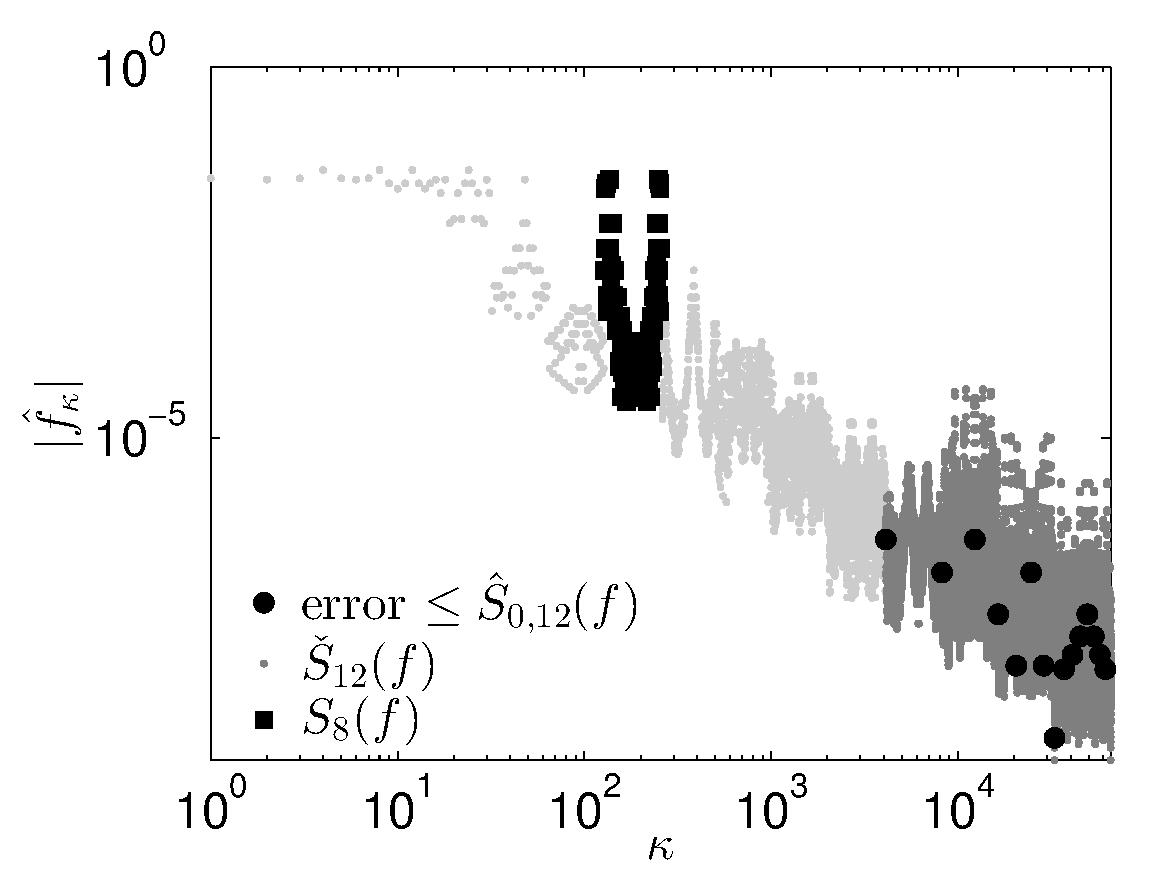
\includegraphics[width=9cm]{Images/PlotFFTCoefUse256.eps}
\caption{The magnitudes of true Fourier coefficients for some integrand. \label{Walshcoeffig}}
\end{figure}

Because we do not assume the knowledge of the true  Fourier  coefficients, for functions in $\cc$ we need bounds on $S_{\ell}(f)$ in terms of the sum of the discrete coefficients $\tS_{\ell,m}(f)$.  This is done by applying \eqref{tfassumc},  and the definition of the cone in \eqref{conecond}:
\begin{align}
\nonumber
S_\ell(f) &= \sum_{\kappa=b^{\ell-1}}^{b^{\ell}-1} \bigl \lvert \hf_{\kappa}\bigr\rvert= \sum_{\kappa=b^{\ell-1}}^{b^{\ell}-1} \abs{\tf_{m,\kappa} - \sum_{\lambda=1}^{\infty} \hf_{\kappa+\lambda b^{m}} \E^{2 \pi \sqrt{-1} \ip{\tvk(\kappa+\lambda b^{m}) \ominus \tvk(\kappa)}{\bsDelta}}}\\
\nonumber
&\le \sum_{\kappa=b^{\ell-1}}^{b^{\ell}-1} \bigl \lvert \tf_{m,\kappa} \bigr\rvert + \sum_{\kappa=b^{\ell-1}}^{b^{\ell}-1} \sum_{\lambda=1}^{\infty} \bigl \lvert \hf_{\kappa+\lambda b^{m}}\bigr\rvert = \tS_{\ell,m}(f) + \hS_{\ell,m}(f) \\
\label{boundSumbsApproxa}
&\le \tS_{\ell,m}(f) + \homega(m-\ell) \wcomega(m-\ell) S_\ell\
\end{align}
and provided that $\homega(m-\ell) \wcomega(m-\ell)<1$,
\begin{equation}\label{boundSumsApproxb}
S_\ell(f) \le \frac{\tS_{\ell,m}(f)}{1 - \homega(m-\ell) \wcomega(m-\ell)}.
\end{equation}
By \eqref{err2} and the cone conditions, the above inequality implies a data-based error bound:
\begin{align}
\nonumber
\biggabs{\int_{\cube} f(\bsx) \, \D \bsx - \hI_m(f) }
&\le \sum_{\lambda=1}^{\infty} \bigabs{\hf_{\lambda b^{m}}} 
= \hS_{0,m}(f)\le \homega(m) \wcS_m(f)\\
\nonumber
&  \le \homega(m) \wcomega(m-\ell) S_\ell(f)\\
& \le  \frac{\homega(m) \wcomega(m-\ell)}{1 - \homega(m-\ell) \wcomega(m-\ell)}\tS_{\ell,m}(f)
\label{SSbd2}
\end{align}
Based on this conservative bound an adaptive algorithm is constructed in the next Section. 

\section{An Adaptive Algorithm Based for Cones of Integrads}\label{algorithmsection}

Inequality \eqref{SSbd2} suggests the following algorithm. First, choose $\ell_*$ and fix $r:=m-l \in \N$ such that $\homega(r)\wcomega(r)<1$ for $\ell\geq\ell_*$. Then, define
\[
\fC(m):= \frac{\homega(m) \wcomega(r)}{1 - \homega(r) \wcomega(r)}.
\]

The choice of the parameter $r$ is important. Larger $r$ means a bigger $\fC(m)$ although makes the error more dependent on smaller indexed Fourier coefficients.

\begin{algo}[Adaptive Rank-1 Lattice Cubature, \texttt{cubLattice\_g}] \label{adapalgo} Fix $r$, $\ell_*$ as described above and $\homega$ and $\wcomega$ describing $\cc$ in \eqref{conecond}. Given a tolerance, $\varepsilon$, initialize $m=\ell_*+r$ and do the following:

\begin{description}
\item[\textbf{Step 1.}] According to Section \ref{FFT}, compute $\tS_{m-r,m}(f)$.
\item[\textbf{Step 2.}] Check whether $\fC(m)  \tS_{m-r,m}(f) \le \varepsilon$. If true, return $\hI_m(f)$ defined in \eqref{cubaturedef}. If not, increment $m$ by one, and go to Step 1.
\end{description}
\end{algo}

\begin{theorem} \label{adapalgothm} For $m = \min \{m' \ge \ell_*+r : \fC(m')  \tS_{m'-r,m'}(f) \le \varepsilon \}$, Algorithm \ref{adapalgo} is successful whenever $f\in\cc$,
\[
\biggabs{\int_{\cube} f(\bsx) \D \bsx - \hI_m(f)} \le \varepsilon.
\]
Thus, the number of function data needed is $b^m$. Defining $m^* = \min \{m' \ge \ell_*+r : \fC(m') [1+ \homega(r) \wcomega(r)] S_{m'-r}(f) \le \varepsilon \}$, we also have $b^m\leq b^{m^*}$. This means that the computational cost can be bounded,
\[
\mathrm{cost}\left(\widehat{I}_m,f,\varepsilon\right)\leq \$(f)b^{m^*}+cm^*b^{m^*}
\]
where $\$(f)$ is the cost of evaluating $f$ at one data point.
\end{theorem}

\begin{proof}
By construction, the algorithm must be successful. Recall that the inequality used for building the algorithm is \eqref{SSbd2}.

In order to find the upper bound on the computational cost one can obtain, analogously to the result in \eqref{boundSumbsApproxa},
\begin{align}
\nonumber
\tS_{\ell,m}(f) &= \sum_{\kappa=b^{\ell-1}}^{b^{\ell}-1} \bigabs{ \tf_{m,\kappa}} = \sum_{\kappa=b^{\ell-1}}^{b^{\ell}-1} \biggabs{\hf_{\kappa} + \sum_{\lambda=1}^{\infty} \hf_{\kappa+\lambda b^{m}} \E^{2 \pi \sqrt{-1} \ip{\tvk(\kappa+\lambda b^{m}) \ominus \tvk(\kappa)}{\bsDelta}}}\\
\nonumber
&\le \sum_{\kappa=b^{\ell-1}}^{b^{\ell}-1} \bigabs{\hf_{\kappa}} + \sum_{\kappa=b^{\ell-1}}^{b^{\ell}-1} \sum_{\lambda=1}^{\infty} \bigabs{\hf_{\kappa+\lambda b^{m}}} 
= S_{\ell}(f) + \hS_{\ell,m}(f) \\
\nonumber
&\le [1  + \homega(m-\ell) \wcomega(m-\ell)] S_\ell(f). \label{SSbd3}
\end{align}
Replacing $\tS_{\ell,m}(f)$ in the error bound in \eqref{SSbd2} by the right hand side above proves that the choice of $m$ needed to satisfy the tolerance is no greater than  $m^*$ defined above.

In Section \ref{FFT}, the computation of $\tS_{m-r,m}(f)$ is described in terms of $\Order(mb^m)$ operations. Thus, the total cost of Algorithm \ref{adapalgo} is,
\[
\mathrm{cost}\left(\widehat{I}_m,f,\varepsilon\right)\leq \$(f)b^{m^*}+cm^*b^{m^*}
\]
\hfill \qed
\end{proof}

\section{Numerical Example} \label{secnumexpsec}

Algorithm \ref{adapalgo} has been coded in MATLAB as \texttt{cubLattice\_g} in base 2, and is scheduled to appear in the next release for the Guaranteed Automatic Integration Library, \cite{ChoEtal14a}. For testing it, we priced an Asian call with geometric Brownian motion, $S_0=K=100$, $T=1$ and $r=3\%$. The test is performed on 500 samples whose dimensions are chosen IID uniformly among 1, 2,4,8,16,32 and 64, and the volatility also IID uniformly from $10\%$ to $70\%$. Results, in Figure \ref{geoAsianmean}, show $97\%$ of success meeting the error tolerance.

The algorithm parametrization according to the cone chosen by default was $\ell_*=6$, $r=4$ and $\fC(m)=5 \times 2^{-m}$. However, the results are strongly dependent on the generating vector that was used for creating the rank-1 lattice embedded node sets. The vector applied to this example was found with the \texttt{latbuilder} software from Pierre L'Ecuyer and David Munger \cite{????}, in the special case of $n=2^{26}$ points, $d=250$ and weights $\gamma_j=j^{-2}$. The best choice of generating vector for \texttt{cubLattice\_g} needs further research.

\begin{figure}[h!]
\centering
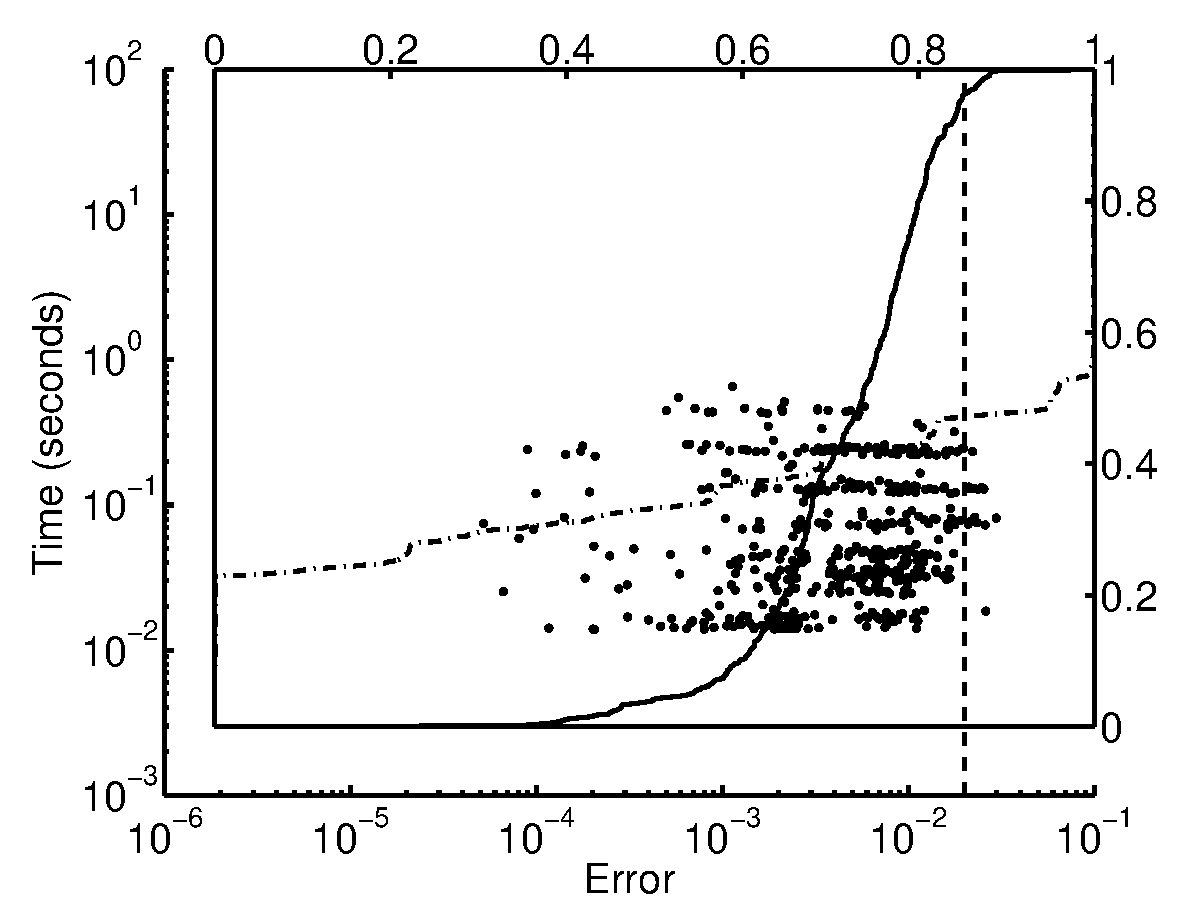
\includegraphics[width=7cm]{Images/geomeancubLatticeErrTime_d_64.eps} 
\caption{Empirical distribution functions obtained from 500 samples, for the error (continuous line) and time (slashed-doted line). The vertical slashed line represents the tolerance 0.02 in each sample. \label{geoAsianmean}}
\end{figure}

\section{Discussion and Future Work}
Quasi-Monte Carlo methods rarely provide guaranteed and adaptive algorithms. Developing a new methodology to bound the absolute error via the discrete Fourier coefficients has allowed us to build an adaptive automatic algorithm guaranteed for cones of integrands. The definition of cone is a challenging new viewpoint whose non-convexity leads to a nonlinear algorithm, and the complexity of the integration problem over this set may be hard to analyze. Our algorithm provides an upper bound on the complexity, but we have not yet obtained a  lower bound. In the future, we also hope to link this work to other results provided in the literature by drawing a correspondence between our cone of integrands and more common spaces of integrands, like the Korobov spaces. Finally, we are also interested in extending our algorithm to accommodate  a relative error tolerance and study the impact of the dimension in it as well as establishing the best generating vector.

\begin{acknowledgement}
The authors thank Ronald Cools and Dirk Nuyens for organizing MCQMC 2014 and greatly appreciate the suggestions made by Sou-Cheng Choi, Frances Kuo, Lan Jiang, Dirk Nuyens and Yizhi Zhang to improve this manuscript. In addition, the first author also thanks Art Owen for partially funding traveling expenses to MCQMC 2014.
This work was partially supported by US National Science Foundation grants DMS-1115392 and DMS-1357690. 
\end{acknowledgement}

\bibliographystyle{spmpsci.bst}
\bibliography{FJH22,FJHown23,lluisantoni}

\end{document}



This map has the desirable property of identifying those wavenumbers, $\bsk$, with the corresponding index in the fast Fourier transform.  This next lemma provides some properties of this map.

\begin{lemma} \label{numaplem} The following is true for the map in Definition \ref{numapdef}:  for all $m \in \N_0$
\begin{enumerate}
\item $\tnu_m(\bszero) = 0$;
\item $\hnu_m(\bsk)\in \F_b$ and $\tnu_m(\bsk)\in \F_{b^m}$;
\item for all $m\in \N_0$ and all $\bsnu \in \F_b^{m}$ there exist a unique $\bsk \in \Z^d$ with $\hbsnu(\bsk)=(\nu_0, \ldots, \nu_{m-1}, \ldots)$.
\item for any $m \in \N_0$, $i \in \{0, \ldots, b^m-1\}$,  $\tnu_m(\bsk)=\nu=(\nu_0, \nu_1, \ldots)$, and $\bsi=(i_0, i_1, \ldots)$, it follows that
\begin{align} \label{nuwisum}
\begin{split}
\ip{\bsk}{\bsz_i} &= \sum_{\ell=0}^{m-1} i_\ell [\nu \bmod  {b^{(l+1)}}]  b^{-(l+1)} \bmod 1
\end{split}
\end{align}

\end{enumerate}
\end{lemma}

\begin{proof}
\begin{enumerate}
\item Directly from definition.
\item Using \eqref{latpropc} and by construction, $\hnu_0(\bsk)\in\{0,\dots,b-1\}$ and $\hnu_m(\bsk)\in (-1,b)$. Using the assumption \eqref{latpropb}, $\hnu_m(\bsk)\bmod 1=\bsk^Tb\bsz_{b^m}\bmod 1-\bsk^T\bsz_{b^{m-1}}\bmod 1=0$. Then, $\hnu_m(\bsk)\in (-1,b)\cap\Z=\{0,\dots,b-1\},\;\forall m\in\N_0$.

\item For injection, we are proving that $\hbsnu(\bsk)=\hbsnu(\bsl) \Rightarrow \bsk = \bsl$. If $\hbsnu(\bsk)=\hbsnu(\bsl)$, $\hnu_m(\bsk)=\hnu_m(\bsl),\;\forall m\in\N_0$. In particular for $m=0$, this implies $\ip{\bsk}{\bsz_1}-\ip{\bsl}{\bsz_1}=0$. Recursively, one obtains that $\ip{\bsk}{\bsz_{b^m}}-\ip{\bsl}{\bsz_{b^m}}=0$. Therefore, $\ip{\bsk}{\bsz_{b^{m}}}-\ip{\bsl}{\bsz_{b^{m}}}=\ip{\bsk-\bsl}{\bsz_{b^{m}}}=0$ for all $m\in\N_0$ and by \eqref{latpropd}, $\bsk=\bsl$.

For surjection, by \eqref{bilinearlinzeroprop} there exists $\bsk$ such that $\hnu_0(\bsk)=\nu\neq 0$. Furthermore due to the property \eqref{bilinearlinkprop}, $\hnu_0(a\bsk)=a\nu \bmod b$ and recalling the Lagrange's Theorem, any element $\nu$ different than the identity generates the group $\F_b$. Therefore, for $a=1,\dots,b-1$ we can obtain all elements in $\F_b$. Now, for any $\ell\leq m\in\N$ and using \eqref{assumgenip},
\begin{align*}
\hnu_\ell(\bsk+b^m\bsa)&=
\begin{cases}
b\ip{\bsk}{\bsz_{b^\ell}}-\ip{\bsk}{\bsz_{b^{\ell-1}}}+b\ip{\bsa}{\bsz_{1}} \bmod b  &\mbox{if } \ell=m, \\
b\ip{\bsk}{\bsz_{b^\ell}}-\ip{\bsk}{\bsz_{b^{\ell-1}}} &\mbox{if } \ell<m   \end{cases}\\
&=
\begin{cases}
\hnu_\ell(\bsk)+\hnu_0(\bsa) \bmod b  &\mbox{if } \ell=m, \\
\hnu_\ell(\bsk) &\mbox{if } \ell<m   \end{cases}\\
\end{align*}%Remark that for the first equality we use the fact that $\ip{\bsk}{\bsz_{b^{m-1}}}=\ip{\bsk}{\bsz_{b^{m-1}}}\bmod b$. 
Therefore, for all $m\in \N_0$ and all $(\nu_0,\dots,\nu_m) \in \F_b^{m+1}$ one can build recursively $\bsk \in \Z^d$ such that  $\hnu_\ell(\bsk)=\nu_\ell$, $\ell=0,\dots,m$.

\item Directly by applying \eqref{bilinearlinxprop} and Definition \ref{numapdef}:
\begin{align*}
\ip{\bsk}{\bsz_i} &= \ip{\bsk}{\sum_{\ell=0}^{m-1} i_\ell \bsz_{b^{\ell}}} = \sum_{\ell=0}^{m-1} i_\ell \ip{\bsk}{\bsz_{b^{\ell}}} \bmod 1 \\
& = \sum_{\ell=0}^{m-1} i_\ell \sum_{j=0}^{\ell} \nu_jb^{j-(\ell+1)} \bmod 1\\
&=\sum_{\ell=0}^{m-1} i_\ell [\nu \bmod  {b^{(\ell+1)}}]  b^{-(\ell+1)} \bmod 1.
\end{align*}
\end{enumerate}
\hfill\qed
\end{proof}

To explain the hidden constraint in this mapping, we need to define the dual cosets. Given the dual lattice $\cp_{m}^{\perp}$, for $m\in\N_0$ one can find another $b^m-1$ cosets redefining \eqref{dualdef},
\begin{align}
\cp_{m,c_m}^\perp:=\{\bsk \in \Z^d : \ip{\bsk}{\bsz_{b^{\ell}}} = c_m/b^m, \ \ell=0, \ldots, m-1\}, \; c_m=0, \ldots, b^m-1.\label{dualdefcoset}
\end{align}
Here, $\cp_{m}^{\perp}=\cp_{m,0}^\perp$ and the embedded structure described earlier in \eqref{dualemb} is inherited for any coset:
\begin{equation}\label{dualemb}
\Z^d=\cp^{\perp}_{0,0}\supseteq\dots\supseteq\cp^{\perp}_{m,c_m}\supseteq\dots\supseteq\cp^{\perp}_{\infty}=\{0\}.
\end{equation}
Therefore, in order to preserve this structure, Definition \ref{wavenummapdef} obliges that
\begin{equation}
\cp^{\perp}_{m,c_m}=\bigoplus_{a=0}^{b-1}\cp^{\perp}_{m+1,c_m+ab^m}, \qquad m\in\N_0.
\end{equation}